\appendices

%\section{Attack Sequence of pNetwork Hack}

%\Cref{fig:sqeuence} shown the attack sequence of pNetwork attack.
%\label{pnetwork_sequence}
\section{真实世界攻击示例}

\subsection{本文分类中五类攻击向量的示例}
\label{appendix:examples}

\paragraph{事件仿冒}
\emph{事件仿冒}的两个知名实例是针对 Qubit Bridge~\cite{Qubit} 和 Meter Bridge~\cite{Meter} 的攻击，分别造成了 8000 万美元和 430 万美元的损失。

\paragraph{不一致日志记录}
许多此类问题是在 2024 年 4 月 1 日对 BSC 链上最活跃的 25 个智能合约进行分析时发现的。具体而言，TroyEmpire~\cite{TroyEmpire}、SecondLive~\cite{SecondLive}、WalletLocking~\cite{WalletLocking} 和 TTGameEvents~\cite{TTGame} 的合约被发现存在这些问题。例如，TTGame 项目会为用户注册生成一个地址，并向该地址转入一定数量的 BNB，作为未来自动调用所需的 gas 费用。通过从历史交易中识别授权用户地址，我们可以发现其余发出幻影事件的未授权交易。尽管其他三个项目的用户权限并不明确，但我们可以通过模拟调用它们的函数任意生成取款事件，从而确认这些问题的存在。

\paragraph{合约仿冒}
对于\emph{合约仿冒}攻击，最显著的实例是针对 pNetwork 的攻击，该攻击造成了 1270 万美元损失。该案例已在\cref{sec:motivation}中作了简要介绍。类似地，THORChain 也因错误处理器问题遭受了 800 万美元损失~\cite{thorchain}。至于仿冒合约攻击，一个代表性案例是 ``sleepminting'' 攻击，该攻击因生成一个价值 6900 万美元的 NFT 并将其上架到平台而受到关注。该事件已在学术界得到广泛研究~\cite{nft_sleepminting,clone_nft,sleepminting}。根据 Forta 平台近期信息~\cite{sleepminting_forta}，在 2023 年 12 月 3 日至 12 月 9 日短短 7 天内，就生成了 8,130 条 sleepminting 告警。

\paragraph{转账事件欺骗}
我们对链上数据的分析揭示了大量\emph{转账事件欺骗}实例，其中 ERC-20 代币和 NFT 事件的发送者地址被篡改。这些实例包括类似名人、知名交易所和其他吸引注意力实体的伪造地址。其中若干案例已导致重大经济损失~\cite{layerzero_scam,TetherClaims,ethaddress,zero_transfer,wallet_visual}。

\paragraph{事件处理错误}
\emph{事件处理错误}的一个知名示例是 Rarible 和 OpenSea 因 sleepminting 遭遇的错误信息展示案例。Etherscan 和 Bscscan 等区块链浏览器以及各种钱包，常常会将伪造转账事件视为合法交易。另一个实例涉及 blockwell.ai，其中钱包错误地将来自欺骗代币的幻影事件识别为有效 ERC-20 转账~\cite{blockwell.ai}。在 ERC-721 和 ERC-1155 代币中也观察到了类似漏洞。

此外，最大的 NFT 市场 OpenSea 也曾面临类似问题。攻击者操纵 OpenSea 所显示 NFT 的元数据，并嵌入恶意载荷以触发非预期的钱包行为，最终使攻击者获利。类似攻击也出现在 ERC-20 项目中，这凸显了整个区块链生态系统在安全处理事件数据方面所面临的普遍困难~\cite{rektosaurus,OpenSea}。

\subsection{不一致日志记录与合约仿冒框架}

\begin{figure}
    \centering
    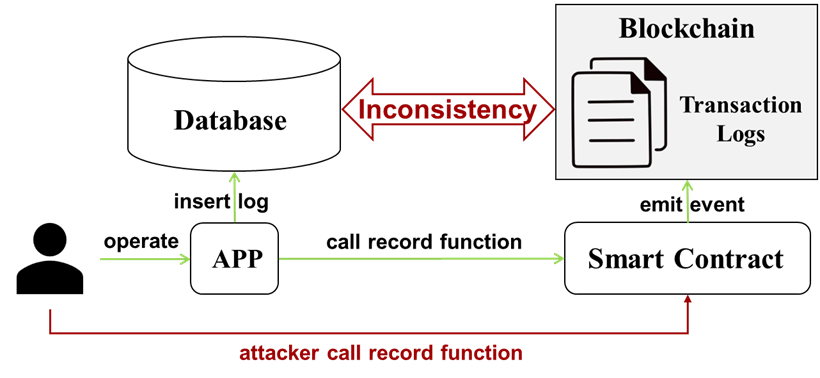
\includegraphics[width=1\linewidth]{Sections//Picture/inconsistency.png}
    \caption{不一致日志记录应用概览。}
    \label{fig:Inconsistent_logging}
\end{figure}

~\Cref{fig:Inconsistent_logging} 给出了应用中\emph{不一致日志记录}的概览。在该框架中，用户通过应用进行操作，应用一方面与数据库交互以插入日志，另一方面与区块链上的智能合约交互以发出事件。然而，由于日志记录实践存在差异，数据库日志和区块链交易日志之间可能出现不一致。攻击者可以通过直接调用记录函数来利用这一点，从而可能在应用内部日志记录与区块链交易日志之间制造不匹配。

\begin{figure}[!htbp]
    \centering
    \begin{subfigure}[b]{0.5\textwidth}
        \centering
        
\includegraphics[width=\textwidth]{Sections/Picture/attack1-1.png}
        \caption{混合事件攻击}
        \label{fig:attack3-1}
    \end{subfigure}
    \quad
    \begin{subfigure}[b]{0.5\textwidth}
        \centering
        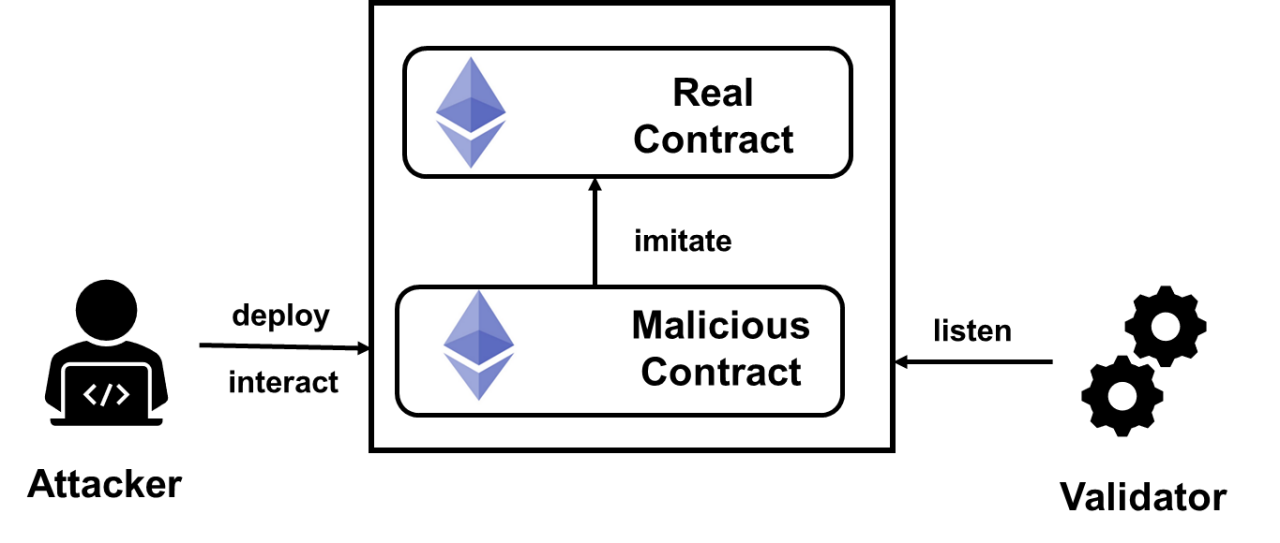
\includegraphics[width=\textwidth]{Sections/Picture/attack1-2-0.png}
        \caption{仿冒合约攻击}
        \label{fig:attack3-2}
    \end{subfigure}
    \caption{两类合约仿冒}
    \label{fig:attack1}
\end{figure}

~\Cref{fig:attack1} 展示了两类合约仿冒攻击。在\emph{混合事件攻击}中，恶意合约与真实合约交互，两个合约的日志被记录在同一笔交易中，这可能误导验证者。在\emph{仿冒合约攻击}中，攻击者部署一个模仿真实合约的合约，生成看似源自真实合约的欺骗性日志，进一步干扰验证者判断。

\subsection{转账事件欺骗案例}

\begin{figure}
    \centering
    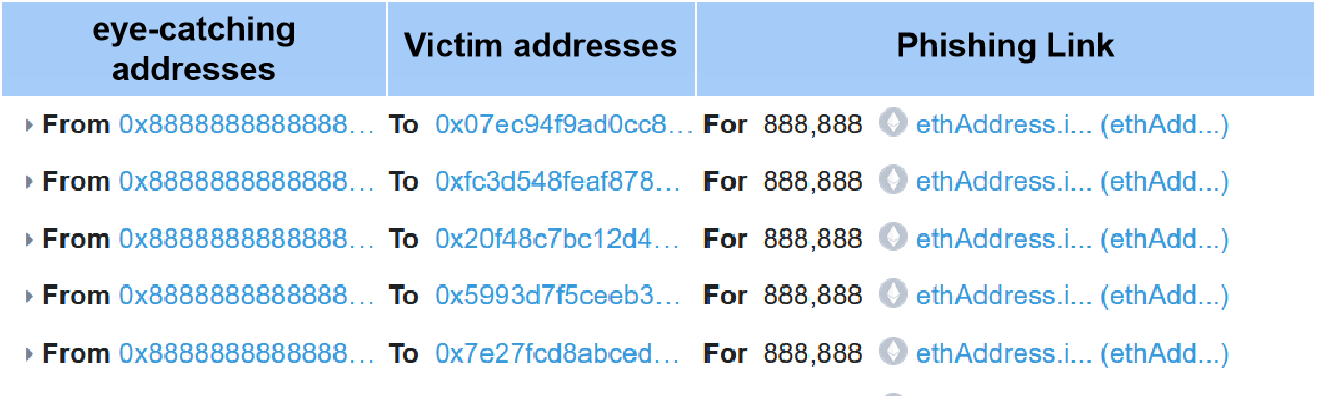
\includegraphics[width=1\linewidth]{Sections//Picture/address.png}
    \caption{空投事件欺骗。}
    \label{fig:airdrop}
\end{figure}

~\Cref{fig:airdrop} 展示了一个\emph{转账事件欺骗}攻击示例，其中攻击者伪造事件发送者，导致区块链浏览器和钱包错误地将其显示为一次成功转账。这种错误展示可能欺骗用户，并被用作一种社会工程学手段，以利用用户对这些界面的信任。


% \section{Real case of transfer event spoofing attack transactions.}
\begin{table}[]
\caption{转账事件欺骗攻击交易的真实案例。}
\label{tab:transfer_spoof_attack_transaction}
\begin{tabular}{lllll}
\toprule
  & 发送者 & 转账来源                & 转账去向                  & 代币      \\
\midrule
1 & Victim           & Victim & 0x{\color[HTML]{FE0000}734}659...50C{\color[HTML]{FE0000}a79F7} & USDT \\
\midrule
2 & Attacker              & Victim & 0x{\color[HTML]{FE0000}734}35A..2Bc{\color[HTML]{FE0000}a79F7}  & FAKE USDT     \\
\midrule
3 & Victim           & Victim & 0x{\color[HTML]{FE0000}734}35A...2Bc{\color[HTML]{FE0000}a79F7} & USDT \\
\bottomrule
\end{tabular}
\end{table}
2024 年 2 月 9 日发生的\emph{转账欺骗}攻击中，攻击者成功执行了一次\emph{转账事件欺骗}攻击，造成 104 万美元损失。该攻击利用了钱包和区块链浏览器在解析和显示转账事件时存在的漏洞。如\Cref{tab:transfer_spoof_attack_transaction}所示，在用户向合法地址（0x734\ldots{}a79F7）发送资金后，攻击者伪造了一个转账事件，使其看起来像是资金被发送到了一个由攻击者控制的相似地址。由于某些钱包和浏览器处理这些事件的方式存在问题，该虚假转账被显示为合法交易，导致用户误将额外资金发送到攻击者地址，造成重大经济损失~\cite{zero_transfer}。
